\chapter{实现保护模式}\label{cha:latex-brief-intro}
为了使实验报告清晰简洁,后续实验均省略了部分具体代码实现部分,仅重点说明主要数据和代码结构,以体现设计的核心思想。

\section{实验内容}
认识保护模式,实现从实模式到保护模式的转换,GDT 描述符;实现实模式大于 1MB 内存的寻址能力,并接着上一次实验,从保护模式返回到实模式,重新设置各个段寄存器的值;LDT 描述符;学会使用挂载指令和运行程序。

\section{代码分析}

\subsection{核心数据结构}

\begin{table}[H]
\begin{center}
\caption{[SECTION .gdt]段 gdt数据段}
\begin{tabular}{|c|ll|}
\hline
\multirow{3}{*}{数组 GDT} & \multicolumn{2}{l|}{LABEL\_GDT 空描述符}                 \\ \cline{2-3} 
                        & \multicolumn{2}{l|}{LABEL\_DESC\_CODE32 非一致代码段32描述符} \\ \cline{2-3} 
                        & \multicolumn{2}{l|}{LABEL\_DESC\_VIDEO 显存首地址}        \\ \hline
\multirow{2}{*}{变量}     & \multicolumn{2}{l|}{Gdtlen 表示GDT的长度}                 \\ \cline{2-3} 
                        & \multicolumn{2}{l|}{GdtPtr dw为GDT界限 dd为GDT基址}        \\ \hline
\multirow{2}{*}{选择子}    & \multicolumn{2}{l|}{SelectorCode32 非一致代码段32选择子}      \\ \cline{2-3} 
                        & \multicolumn{2}{l|}{SelectorVideo 视频段选择子}            \\ \hline
\end{tabular}
\end{center}
\end{table}
如表 4-1 所示,该部分对应“认识保护模式,实现从实模式到保护模式的转换,认识 GDT 描述符,并进入保护模式”的数据结构。

\begin{table}[H]
\begin{center}
    \caption{[SECTION .gdt]段 gdt数据段}
\begin{tabular}{|c|l|l|}
\hline
\multirow{8}{*}{数组 GDT}                 & LABEL\_GDT          & 空描述符                       \\ \cline{2-3} 
                                        & LABEL\_DESC\_NORMAL & Normal 描述符                 \\ \cline{2-3} 
                                        & LABEL\_DESC\_CODE32 & 非一致代码段 32 描述符              \\ \cline{2-3} 
                                        & LABEL\_DESC\_CODE16 & 非一致代码段 16 描述符              \\ \cline{2-3} 
                                        & LABEL\_DESC\_DATA   & 数据段描述符                     \\ \cline{2-3} 
                                        & LABEL\_DESC\_STACK  & 32 位堆栈段描述符                 \\ \cline{2-3} 
                                        & LABEL\_DESC\_TEST   & 测试段描述符                     \\ \cline{2-3} 
                                        & LABEL\_DESC\_VIDEO  & 显存描述符                      \\ \hline
\multirow{2}{*}{变量}                     & Gdtlen              & 表示 GDT 的长度                 \\ \cline{2-3} 
                                        & GdtPtr              & \begin{tabular}
                                                                [c]{@{}l@{}}前两个字节为GDT界限\\ 
                                                                后四个字节为GDT基址\end{tabular} \\ \hline
\multirow{2}{*}{选择子}                    & SelectorNormal      & Normal 选择子                 \\ \cline{2-3} 
                                        & SelectorCode32      & 非一致代码段 32 选择子              \\ \hline
\multicolumn{1}{|l|}{\multirow{5}{*}{}} & SelectorCode16      & 非一致代码段 16 选择子              \\ \cline{2-3} 
\multicolumn{1}{|l|}{}                  & SelectorData        & 数据段选择子                     \\ \cline{2-3} 
\multicolumn{1}{|l|}{}                  & SelectorStack       & 堆栈段选择子                     \\ \cline{2-3} 
\multicolumn{1}{|l|}{}                  & SelectorTest        & 测试段选择子                     \\ \cline{2-3} 
\multicolumn{1}{|l|}{}                  & SelectorVideo       & 视频段选择子                     \\ \hline
\end{tabular}
\end{center}
\end{table}

\begin{table}[H]
\begin{center}
\caption{[SECTION .data1] 数据段}
\begin{tabular}{|c|l|l|}
\hline
\multirow{6}{*}{常量} & SPValueInRealMode & 字符串                                                                     \\ \cline{2-3} 
                    & PMMessage         & 在保护模式中显示的信息"In Protect Mode now. \textasciicircum{}-\textasciicircum{}" \\ \cline{2-3} 
                    & OffsetPMMessage   & PMMessage 段偏移                                                           \\ \cline{2-3} 
                    & StrTest           & “ABCDEFGHIJKLMNOPQRSTUVWXYZ”                                            \\ \cline{2-3} 
                    & OffsetStrTest     & StrTest 段偏移                                                             \\ \cline{2-3} 
                    & DataLen           & 表示数据段的长度                                                                \\ \hline
\end{tabular}
\end{center}
\end{table}

\begin{table}[H]
\begin{center}
\caption{[SECTION .gs] 全局堆栈段}
\begin{tabular}{|c|l|l|}
\hline
常量 & TopOfStack & 栈顶指针 \\ \hline
\end{tabular}
\end{center}
\end{table}

如表 4-2、4-3、4-4 所示,该部分对应“实现实模式大于 1MB 内存的寻址,并接着上一次实验,在 DOS 模式下从保护模式返回到实模式,重新设置各个段寄存器的值”的数据结构。

\begin{table}[H]
\begin{center}
\caption{[SECTION .ldt]段 LDT数据段}
\begin{tabular}{|c|l|l|}
\hline
\multirow{3}{*}{LDT 数组} & LABEL\_LDT\_DESC\_CODEA & LDT 描述符    \\ \cline{2-3} 
                        & LDTLen                  & 表示 LDT 的长度 \\ \cline{2-3} 
                        & SelectorLDTCodeA        & LDT 选择子    \\ \hline
\end{tabular}
\end{center}
\end{table}

如表 4-2、4-3、4-4、4-5 所示,该部分对应“了解 LDT 描述符;学会使用挂载指令将文件挂载在临时目录和并运行程序”的数据结构。

\subsection{关键代码段分析}
\begin{enumerate}
    \item \texttt{[SECTION .s16][BITS 16]} --- 代码段:从实模式跳到保护模式
    \begin{itemize}
        \item 初始化 32 位代码段描述符:将 \texttt{[SECTION .S32]} 段的物理地址分三部分赋给空白描述符 \texttt{DESC\_CODE32}
        \item 为加载 \texttt{GDTR} 做准备:将 \texttt{GDT} 的物理地址填充到 \texttt{GdtPtr} 中
        \item 加载 \texttt{GDTR}:将 \texttt{GdtPtr} 加载到寄存器 \texttt{gdtr} 中
        \item 关中断
        \item 打开 \texttt{A20} 地址线:通过操作端口 \texttt{92h}
        \item 准备切换到保护模式:把寄存器 \texttt{cr0} 的第 0 位置为 1
        \item 进入保护模式:\texttt{Jump}
    \end{itemize}
    
    \item \texttt{[SECTION .s32][BITS 32]} --- 32 位代码段,由实模式跳入。将视频段选择子 \texttt{SelectorVideo} 的地址赋给 \texttt{gs}
    \begin{itemize}
        \item 设置输出位置为屏幕 11 行 79 列
        \item 设置输出为黑底红字
        \item 往显存中 \texttt{edi} 偏移处写入 \texttt{P}
        \item 无限循环
    \end{itemize}
    
    \item 从保护模式跳回到实模式
    \begin{itemize}
        \item 程序重设各个段寄存器值,使 \texttt{ds}、\texttt{es}、\texttt{ss} 指向 \texttt{as}
        \item 恢复 \texttt{sp} 的值
        \item 关闭 \texttt{A20}
        \item 打开中断
        \item 回到 DOS
    \end{itemize}
    
    \item \texttt{[SECTION .s32]} --- 32 位代码段,由实模式跳入。初始化 \texttt{ds}、\texttt{es}、\texttt{gs}、\texttt{ss}:
    \begin{itemize}
        \item \texttt{ds} 指向数据段
        \item \texttt{es} 指向新增的 5MB 的内存段
        \item \texttt{gs} 指向显存
        \item \texttt{ss} 指向测试段
        \item 显示一个字符串
        \item 调用读内存函数 \texttt{TestRead}
        \item 调用写函数 \texttt{TestWrite}
        \item 调用函数 \texttt{TestRead}
        \item 跳转到 \texttt{[SECTION .s16code]} 代码段的 \texttt{TestRead} 函数
    \end{itemize}
    
    \item \texttt{[SECTION .s16code]} --- 16 位代码段,由 32 位代码段跳入,跳出后到实模式
    \begin{itemize}
        \item 把选择子 \texttt{SelectorNormal} 加载到 \texttt{ds}、\texttt{es}、\texttt{ss}
        \item 清 \texttt{cr0} 的 \texttt{PE} 位,跳回实模式
        \item 跳转到 \texttt{LABEL\_REAL\_ENTRY} 即段 \texttt{[SECTION .s16]} 里
    \end{itemize}
\end{enumerate}


\section{调试过程及运行结果}

在之前的实验过程中,我们将文件写到了引导扇区运行,但引导扇区只有 512 个字节。空间有限。为使程序扩大,可以选择先借用其他操作系统的引导扇区,我们借用 DOS 操作系统,将程序编译成 COM 文件,然后用 DOS 来执行它。第一步需要到 Bochs 官方网站下载一个 FreeDos,解压后将其中的 a.img 复制到我们的工作目录中,并改名为 freedos.img。紧接着,我们需要使用 bximage 生成一个软盘映像,取名为 pm.img。再其次,我们需要修改我们的 bochsrc与上述img文件对应。最后,直接启动 Bochs 开始调试,即可进入 FreeDos 界面,输入 format b 的指令以便格式化 freedos 的 B:盘。格式化及格式化结果如下图 4-1 所示。
\begin{figure}[H]
  \centering
  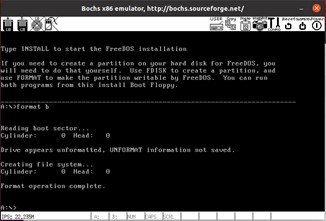
\includegraphics[width=0.8\textwidth]{figures/chapter4/4-1.jpg}
  \caption{freedos格式化B盘示意图}
  \label{fig:1}
\end{figure}

格式化完成后,将上述代码第 8 行中的 07c00h 改为 0100h,并重新编译为 com 文件:
\begin{lstlisting}[language = bash]
  \nasm pmtest1.asm -o pmtest1.com
\end{lstlisting}
紧接着,我们需要输入以下三条指令,将 pmtest1.com 复制到虚拟软盘pm.img 中,所需要的指令如下:
\begin{lstlisting}[language = bash]
  \sudo mount -o loop pmimg /mnt/floppy
  \sudo cp pmtest1.com /mnt/floppy
  \sudo umount /mnt/floppy
\end{lstlisting}
此时若出现挂载点不存在的错误,输入以下指令即可解决:
\begin{lstlisting}
  \sudo mkdir /mnt/floppy
\end{lstlisting}
接下来我们需要重新回到 FreeDos 中(即原先打开的 Bochs 虚拟机),并且输入如下命令:
\begin{lstlisting}[language = bash]
  \b:\pmtest1.com
\end{lstlisting}
pmtest1.com 成功运行。可以注意到,一个红色的字母“P”出现在了屏幕的右侧的中部,这代表调试成功,程序已经进入了保护模式。调试结果如下图 4-2 所示。
\begin{figure}[H]
  \centering
  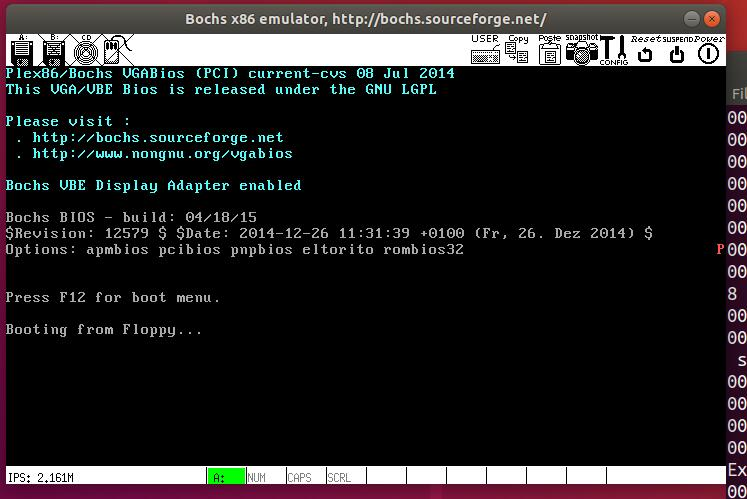
\includegraphics[width=0.8\textwidth]{figures/chapter4/4-2.jpg}
  \caption{pmtest1.com 调试结果}
  \label{fig:2}
\end{figure}

下一步以同样方式运行pmtest2.com。调试结果如下图 4-3 所示,可以看到,程序打印出了两行数字,第一行全部是 0,说明开始内存 5MB 处都是 0,而下一行已经变成了 41、42、43...,说明写操作成功(十六进制的 41、42、43...48 正是 A、B、C...H)。同时可以看到,程序执行结束后没有进入死循环,而是重新出现了 DOS 提示符,这说明我们已经重新到了实模式下的 DOS。
\begin{figure}[H]
  \centering
  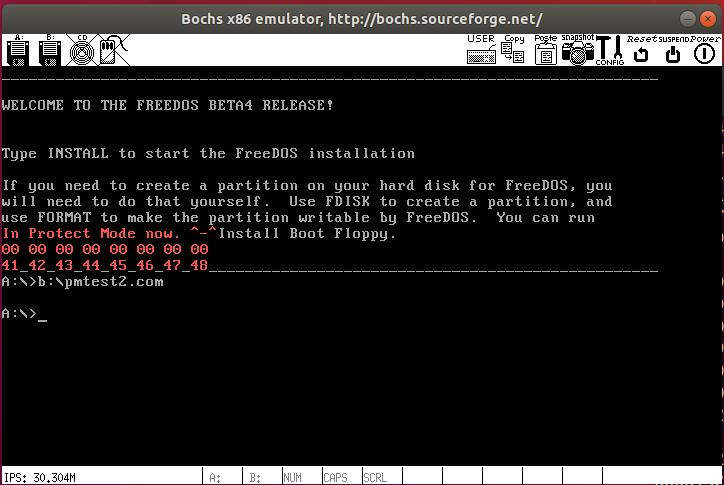
\includegraphics[width=0.8\textwidth]{figures/chapter4/4-3.jpg}
  \caption{pmtest2.com运行结果图}
  \label{fig:3}
\end{figure}

最后再以同样方式运行pmtest3.com。此处 LDT 中的代码段只是打印一个字符 L,因此,在[SECTION .s32]中打印完“In Protect Mode Now.”这个字符串之后,一个红色的字符 L 将会出现。可以看到在下图 4-4 中,的确出现了“In Protect Mode Now.”字符串和一个红色的 L。
\begin{figure}[H]
  \centering
  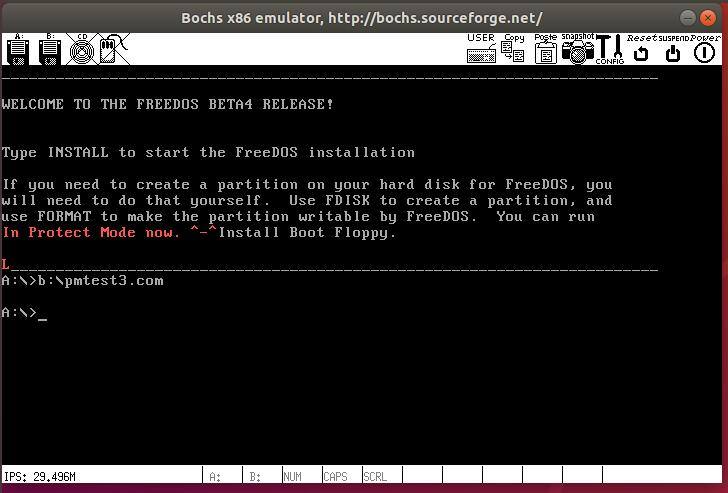
\includegraphics[width=0.8\textwidth]{figures/chapter4/4-4.jpg}
  \caption{pmtest3.com运行结果图}
  \label{fig:4}
\end{figure}

\section{实验总结}

CPU 通常情况下有两种工作模式:实模式和保护模式。打开计算机时CPU默认工作在实模式下,现在需要让其进入保护模式,发挥其寻址能力,并为 32 位系统提供硬件保障。本实验中,在 pm.inc 文件中定义了全局描述表 GDT,定义了相应的段描述符,并且通过 pmtest1.com 由实模式进入保护模式,最后在保护模式中在屏幕右边中央打印了一个红色的“P”,代表实验成功。在调试过程中,我发现只需要将b盘格式化一次,后面就不需要再格式化了。\par
接着,系统成功进入保护模式,打印了一个红色的 P,在本实验中,我们重新建立了一个以 5MB 为基址的段,随后先读出开始处 8 字节的内容,然后写入一个字符串,再从中读出 8 字节。如果读写成功,两次读出的内容不同,而且第二次读出的内容应该前面写进的字符串。然后返回实模式,我们加载了一个合适的描述符选择有关段寄存器,以使对应的段描述符和高速缓存寄存器中含有合适的段界限和属性。而且,我们不能从 32 位代码段返回实模式,只能从 16 位代码段中返回,这是因为无法实现从 32位代码段返回时 cs 高速缓存寄存器中的属性符合实模式的要求(实模式不能改变段属性)。\par
最后,我了解并学习了描述符表LDT,LDT 与 GDT 类似,但它的段选择子的 T1 位必须为 1。类似地,在运用它时,必须先用 lldt 指令加载 ldtr,而 ldtr 的操作数是 GDT 中用来描述 LDT 的段描述符。\par
为了补充相关理论知识,我去查阅相关资料\cite{80286与保护模式}。结合上述实验,我认识到保护模式是 x86 处理器中的一种特殊的操作模式,它与硬件紧密结合,提供了更高级的内存保护和多任务支持。通过将内存划分为多个段并为每个段设置不同的访问权限和保护级别,从而可以防止程序越界访问内存和修改其他程序的数据,提高系统的稳定性和安全性。同时,在保护模式下的操作系统可以实现多任务,每个程序拥有独立的内存空间和代码段,通过任务切换来实现并发执行。结合并发这一点,LDT的引入便显得十分自然,GDT 是全局描述符表,存储了系统中所有进程和任务的段描述符;LDT 是局部描述符表,用于存储特定任务或进程的私有段描述符。通过使用 GDT 和 LDT,操作系统可以对不同任务或进程的内存访问权限进行细粒度控制,提高系统的安全性和灵活性,从而更好地实现并发。
